\documentclass{beamer}

\input{settings.tex}


\title{Interior Point Method}
\subtitle{\mycoursetitle, Lecture 14}
\author{by Sergei Savin}
\centering
\date{\mydate}



\begin{document}
\maketitle


%\begin{frame}{Content}
%
%\begin{itemize}
%	\item Newton method
%	\item Barrier functions
%	\item Interior point method
%	\item Analytic center of linear inequalities
%\end{itemize}
%
%\end{frame}



\begin{frame}{Quadratic Program with One Inequality}
	\begin{flushleft}
		
		We consider:
		\begin{align*}
			\min_{\bo{x}} \quad & \tfrac{1}{2} \bo{x}^\top \bo{Q} \bo{x} + \bo{q}^\top \bo{x} \\
			\text{s.t.} \quad & \bo{A}\bo{x} = \bo{b} \\
			& \bo{c}^\top \bo{x} \le d
		\end{align*}
		
		\vspace{0.5em}
		
		Introduce:
		\begin{itemize}
			\item Slack variable: $z \ge 0$, such that $\bo{c}^\top \bo{x} + z = d$
			\item Dual variables:
			\begin{itemize}
				\item $\bo{y}$ for equality constraint
				\item $s \ge 0$ for inequality constraint
			\end{itemize}
		\end{itemize}
		
		\vspace{0.5em}
		
		Decision variables: $(\bo{x}, \bo{y}, z, s)$
		
	\end{flushleft}
\end{frame}

\begin{frame}{KKT Conditions (Relaxed)}
	\begin{flushleft}
		
		Karush-Kuhn-Tucker (KKT) conditions:
		
		\vspace{0.5em}
		
		\textbf{Stationarity:}
		\[
		\bo{Q}\bo{x} + \bo{q} + \bo{A}^\top \bo{y} + s \bo{c} = 0
		\]
		
		\textbf{Primal feasibility:}
		\[
		\bo{A}\bo{x} = \bo{b}, \quad \bo{c}^\top \bo{x} + z = d
		\]
		
		\textbf{Relaxed complementarity:}
		\[
		z s = \mu
		\]
		
		\textbf{Positivity:}
		\[
		z > 0, \quad s > 0
		\]
		
		\vspace{0.5em}
		
		$\mu > 0$ is the barrier parameter.
		
	\end{flushleft}
\end{frame}


\begin{frame}{Nonlinear System}
	\begin{flushleft}
		
		Define residuals:
		\begin{align*}
			\bo{r}_d &= \bo{Q}\bo{x} + \bo{q} + \bo{A}^\top \bo{y} + s \bo{c} \\
			\bo{r}_p^{(1)} &= \bo{A}\bo{x} - \bo{b} \\
			\bo{r}_p^{(2)} &= \bo{c}^\top \bo{x} + z - d \\
			r_c &= z s - \mu
		\end{align*}
		
		\vspace{0.5em}
		
		We solve the nonlinear system:
		\[
		\bo{r}_d = 0, \quad \bo{r}_p^{(1)} = 0, \quad \bo{r}_p^{(2)} = 0, \quad r_c = 0
		\]
		
	\end{flushleft}
\end{frame}

\begin{frame}{Newton Linearization}
	\begin{flushleft}
		
		Let $(\Delta \bo{x}, \Delta \bo{y}, \Delta z, \Delta s)$ be the Newton step.
		
		\vspace{0.5em}
		
		Linearizing the system:
		
		\vspace{0.5em}
		
		\begin{align*}
			\bo{Q} \Delta \bo{x} + \bo{A}^\top \Delta \bo{y} + \bo{c} \, \Delta s &= -\bo{r}_d \\
			\bo{A} \Delta \bo{x} &= -\bo{r}_p^{(1)} \\
			\bo{c}^\top \Delta \bo{x} + \Delta z &= -\bo{r}_p^{(2)} \\
			s \, \Delta z + z \, \Delta s &= -r_c
		\end{align*}
		
	\end{flushleft}
\end{frame}


\begin{frame}{Step Size Selection}
	\begin{flushleft}
		
		Update:
		\[
		z^+ = z + \alpha \Delta z, \quad s^+ = s + \alpha \Delta s
		\]
		
		\vspace{0.5em}
		
		Choose step size to maintain positivity:
		\[
		z^+ > 0, \quad s^+ > 0
		\]
		
	\end{flushleft}
\end{frame}


\begin{frame}{Barrier Update and Termination}
	\begin{flushleft}
		
		Barrier parameter update:
		\[
		\mu = \sigma (z s), \quad \sigma \in (0,1)
		\]
		
		\vspace{0.5em}
		
		Interpretation:
		\begin{itemize}
			\item $zs$ measures complementarity gap
			\item $\mu \to 0$ drives optimality
		\end{itemize}
		
		\vspace{0.5em}
		
		Termination conditions:
		\begin{itemize}
			\item Primal feasibility: $\|\bo{A}\bo{x} - \bo{b}\|$ small
			\item Inequality feasibility: $|\bo{c}^\top \bo{x} + z - d|$ small
			\item Dual feasibility: $\|\bo{Q}\bo{x} + \bo{q} + \bo{A}^\top \bo{y} + s\bo{c}\|$ small
			\item Complementarity: $zs$ small
		\end{itemize}
		
	\end{flushleft}
\end{frame}


\begin{frame}{Newton method, 1}
	\begin{flushleft}
		
		Given a function $f: \R \rightarrow \R$, we can write it as $y = f(x)$. Consider the problem of finding roots of the equation $f(x) = 0$.
		
		\bigskip
		
		To solve it we can use an iterative procedure. We start at the initial guess $x_0$, produce affine approximation of the function at this point using constant and linear terms of its Taylor expansion:
		
		\begin{equation}
			f = f(x_0) + \frac{\partial f}{\partial x} (x - x_0) + \text{h.o.t.},
		\end{equation}
		
		and then solve the problem $f(x_0) + \frac{\partial f}{\partial x} (x - x_0) = 0$, to find a new point $x_1$, which will serve the role of $x_0$ during the next iteration. This is called \emph{Newton's method}.
		
	\end{flushleft}
\end{frame}


\begin{frame}{Newton method, 2}
	\begin{flushleft}
		
		The solution to the equation $f(x_0) + \frac{\partial f}{\partial x} (x - x_0) = 0$ is:
		
		\begin{equation}
			x = x_0  - \left ( \frac{\partial f}{\partial x} \right )^{-1} f(x_0)
		\end{equation}
		
		\begin{figure}
			\centering
			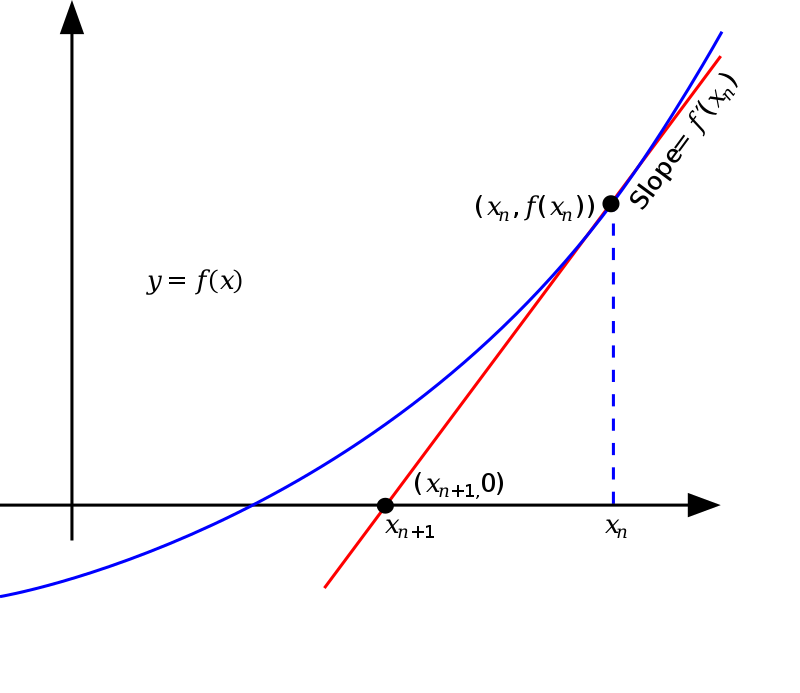
\includegraphics[width=0.6\linewidth]{Newton_iteration}
			\label{fig:newtoniteration}
		\end{figure}
		
		
	\end{flushleft}
\end{frame}



\begin{frame}{Sequantial quadratic approximation, 1}
	\begin{flushleft}
		
		Given a function $\varphi: \R \rightarrow \R$, we can write it as $y = \varphi(x)$. Let us find minimum of this function.
		
		\bigskip
		
		We can try to do it by looking at its quadratic approximation (considering constant, linear and quadratic terms of the Taylor expansion) at an approximation point $x_0$:
		
		\begin{equation}
			\varphi = \varphi(x_0) + \frac{\partial \varphi}{\partial x} (x - x_0)
			+ \frac{1}{2} (x - x_0) \frac{\partial^2 \varphi}{\partial x^2} (x - x_0)
			 + \text{h.o.t.},
		\end{equation}
		%
		and finding its minimum, which can be done by solving a single least-squares problem. Its solution $x_1$ becomes the next approximation point.
		
		\bigskip
		
		This is \emph{another form of the Newton's method}, and is completely equivalent to the previously discussed one. 
		
		
		
	\end{flushleft}
\end{frame}




\begin{frame}{Sequantial quadratic approximation, 2}
	\begin{flushleft}
		
		Let us define $g =\left. \frac{\partial \varphi}{\partial x} \right \vert_{x = x_0}$ and $H = \left. \frac{\partial^2 \varphi}{\partial x^2}\right \vert_{x = x_0}$. Let us solve the problem:
		
		\begin{equation}
			\text{minimize:} \ \ \varphi(x_0) + g (x - x_0)
			+  \frac{1}{2}  (x - x_0) H (x - x_0)
		\end{equation}
		
		The minimum is attained when the derivative is achieves zero:
		
		\begin{equation}
			g + (x - x_0) H = 0
		\end{equation}
		
		This gives us solution $x = x_0 - H^{-1} g$.
		
	\end{flushleft}
\end{frame}





\begin{frame}{Connection of two methods}
	\begin{flushleft}
		
		Let us define a function $p(x) = \frac{\partial \varphi}{\partial x}$. Function $\varphi (x)$ achieves minimum when $p(x)$ crosses zero. Solving the problem $p(x) = 0$ with Newton's method, we initiate iterative process:
		
		\begin{equation}
			x_{i+1} = x_i  - \left ( \frac{\partial p}{\partial x} \right )^{-1} p(x_i)
		\end{equation}
		
		Given the definition of $p(x)$ we can re-write this expression as:
		
		\begin{equation}
			x_{i+1} = x_i  - \left ( \frac{\partial^2 \varphi}{\partial x^2} \right )^{-1} \frac{\partial \varphi}{\partial x}
		\end{equation}
		
		Using previously defined variables $g =\frac{\partial \varphi}{\partial x}$ and $H = \frac{\partial^2 \varphi}{\partial x^2}$ we obtain the same expression we saw in the sequential quadratic approximation:
		%
		\begin{equation}
			x_{i+1} = x_i  - H^{-1} g
		\end{equation}

	\end{flushleft}
\end{frame}





\begin{frame}{Multivariable Newton's method}
	\begin{flushleft}
		
		For mutivaribe case $\varphi: \R^n \rightarrow \R$ the Taylor expansion is given exactly the same:
		%
		\begin{equation}
			\varphi = \varphi(\bo{x}_0) + \frac{\partial \varphi}{\partial \bo{x}} (\bo{x} - \bo{x}_0)
			+ \frac{1}{2} (\bo{x} - \bo{x}_0) \frac{\partial^2 \varphi}{\partial \bo{x}^2} (\bo{x} - \bo{x}_0)
			+ \text{h.o.t.},
		\end{equation}
		
		Solution to the quadratic approximation is given as:
		
		\begin{align}
			\bo{x}_{i+1} &= \bo{x}_i  - \bo{H}^{-1} \bo{g}
			\\
			\bo{x}_{i+1} &= \bo{x}_i  - \left(\frac{\partial^2 \varphi}{\partial \bo{x}^2} \right)^{-1} 
													 \frac{\partial \varphi}{\partial \bo{x}} 
		\end{align}
		
		A key feature of Neuton's method is very fast convergence near the solution.
		
	\end{flushleft}
\end{frame}






\begin{frame}{Solving constrained optimization}
	\begin{flushleft}
		
		Newton's method works for \emph{unconstrained optimization}.
		
		\bigskip
		
		Linear equalities in convex programs can often be excluded by introducing new variables.
		
		\bigskip
		
		Inequality constraints can be replaces with \emph{soft constraints} - an addition to the cost function which punishes decision variables that approach the border of the domain. 
		
	\end{flushleft}
\end{frame}



\begin{frame}{Linear inequalities}
\begin{flushleft}

Consider linear inequality constraints:

\begin{equation}
    \bo{A}\bo{x} \leq \bo{b}
\end{equation}

Remember that we can rewrite it as:

\begin{equation}
    \bo{a}_i^\top \bo{x} \leq b_i
\end{equation}
\begin{equation}
\label{eq:linear_constraints}
    \bo{a}_i^\top \bo{x} - b_i \leq 0
\end{equation}

Instead of \emph{hard constraints} in \eqref{eq:linear_constraints} we can turn these into a cost function component:

\begin{equation}
    J = -\sum\limits_{i = 1}^n \text{log} (b_i - \bo{a}_i^\top \bo{x})
\end{equation}

Which is called a \emph{barrier function}.
 
\end{flushleft}
\end{frame}




\begin{frame}{Barrier functions}
\begin{flushleft}

Let us consider barrier functions $J = -\sum\limits_{i = 1}^n \text{log} (b_i - \bo{a}_i^\top \bo{x})$:

\begin{itemize}
    \item It removes the constraint, but modifies the cost.
    \item When $b_i - \bo{a}_i^\top \bo{x}$ is a very small positive number, $\text{log} (b_i - \bo{a}_i^\top \bo{x})$ is a very big negative number, hence the minus sign in front.
    \item Barrier function does not behave well outside of the domain, when $b_i - \bo{a}_i^\top \bo{x} < 0$.
\end{itemize}
 
\end{flushleft}
\end{frame}




\begin{frame}{Barrier functions for QPs}
\begin{flushleft}

Hence the following QP:

\begin{equation}
\begin{aligned}
& \underset{\bo{x}}{\text{minimize}}
& & \bo{x}^\top \bo{H} \bo{x} + \bo{f}^\top \bo{x}, \\
& \text{subject to}
& & 
\bo{A}\bo{x} \leq \bo{b}
\end{aligned}
\end{equation}
 
...can be approximated as:

\begin{equation}
\begin{aligned}
& \underset{\bo{x}}{\text{minimize}}
& & \bo{x}^\top \bo{H} \bo{x} + \bo{f}^\top \bo{x} - \sum\limits_{i = 1}^n \text{log} (b_i - \bo{a}_i^\top \bo{x})
\end{aligned}
\end{equation}
 
\end{flushleft}
\end{frame}





\begin{frame}{Zero-infinity barrier function}
	\begin{flushleft}
		
		Zero-infinity function can be seen as a precise barrier - adding nothing to the cost in the domain interior and punishing constraint violation by infinite increase of cost:
		
		\begin{equation}
		f(x) = 
		\begin{cases}
			0 &x \leq 0 \\
			\infty &x > 0
		\end{cases}
		\end{equation}
		
		This can be written as max over a family of linear functions:
		
		\begin{equation}
			f(x) = 
			\underset{\lambda \geq 0}{\text{max}}  \  \lambda x
		\end{equation}		
		
		The QP discussed in the previous example becomes:
		
		\begin{equation}
			\begin{aligned}
				& \underset{\bo{x}}{\text{minimize}} \ \underset{\lambda \geq 0}{\text{max}}
				& & \bo{x}^\top \bo{H} \bo{x} + \bo{f}^\top \bo{x} - \sum\limits_{i = 1}^n \lambda_i (b_i - \bo{a}_i^\top \bo{x})
			\end{aligned}
		\end{equation}
		
		It appears that we re-discovered Lagrangian method.
		
		
	\end{flushleft}
\end{frame}




\begin{frame}{Interior point method, 1}
	\begin{flushleft}
		
		Interior point method is based on KKT conditions with a single modification highlifgted below:
		
		\begin{enumerate}
			\item Lagrangian stationarity: $\frac{\partial f_0(\bo{x}) }{\partial \bo{x}} 
			+
			\sum\limits_i 
			\lambda_i  \frac{\partial g_i(\bo{x}) }{\partial \bo{x}} 
			= 0$.
			
			\item Primal feasibility: $g_i(\bo{x}) \leq 0$.
			
			\item Dual feasibility: $\lambda_i \geq 0$.
			
			\item Complementarity slackness: $\lambda_i g_i(\bo{x}) = \textcolor{red}{-\bo{t}_i}$.
		\end{enumerate}
		
		\bigskip
		
		From the complementarity we can find expression for lagrange multipliers:
		
		\begin{equation}
			\lambda_i = -\frac{t_i}{g_i(\bo{x})}
		\end{equation}
		
	\end{flushleft}
\end{frame}




\begin{frame}{Interior point method, 2}
	\begin{flushleft}
		
		Given $\lambda_i = -\frac{t_i}{g_i(\bo{x})}$ we can transform the Lagrangian stationarity condition:
		%
		\begin{equation}
			\frac{\partial f_0(\bo{x})}{\partial \bo{x}} 
			-
			\sum\limits_i 
			\frac{t_i}{g_i(\bo{x})}
			\frac{\partial g_i(\bo{x})}{\partial \bo{x}} 
			= 0
		\end{equation}
		
		Let us compute the following derivative:
		%
		\begin{align}
			\frac{\partial}{\partial \bo{x}} (  -t \log ( -g(\bo{x}) )  ) 
			= \frac{-t}{-g(\bo{x})} (-1) \frac{\partial g(\bo{x})}{\partial \bo{x}} 
			= -\frac{t}{g(\bo{x})} \frac{\partial g(\bo{x})}{\partial \bo{x}} 
		\end{align}
		
		With that, we can re-write the lagrangain condition:
		%
		\begin{equation}
			\frac{\partial f_0(\bo{x})}{\partial \bo{x}} 
			-
			\frac{\partial}{\partial \bo{x}} 
			\left(
			\sum\limits_i 
			t_i \log (- g_i (\bo{x})) 
			\right) = 0
		\end{equation}
		
		
	\end{flushleft}
\end{frame}



\begin{frame}{Interior point method, 3}
	\begin{flushleft}
		
		Condition $\frac{\partial f_0(\bo{x})}{\partial \bo{x}} 
		-
		\frac{\partial}{\partial \bo{x}} 
		\left(
		\sum\limits_i 
		t_i \log (- g_i (\bo{x})) 
		\right) = 0$ is equivalent to minimization:
		
		
		\begin{equation}
			\label{KKT_to_opt}
			\begin{aligned}
				& \underset{\bo{x}}{\text{minimize}}
				& & f_0(\bo{x}) - 
				\sum\limits_i t_i \log (- g_i (\bo{x})) 
			\end{aligned}
		\end{equation}
		
		Solution to this problem $\bo{x}^*$ implies that $\log (- g_i (\bo{x}))$ exists, meaning that $g_i (\bo{x}) \leq 0$, giving us primal feasibility.
		
		\bigskip
		
		In the same way, $\lambda_i = -\frac{t_i}{g_i(\bo{x})} \geq 0$, giving us dual feasibility.
		
		\bigskip
		
		Thus, we have all KKT conditions satisfied automatically by solving the minimization \eqref{KKT_to_opt}.
		
	\end{flushleft}
\end{frame}



\begin{frame}{Interior point method. Central path}
	\begin{flushleft}
		
		\emph{Interior point method} consists of constructing problem \eqref{KKT_to_opt} and solving it using Newton's method for a given value of $t_i$; the method is applied iteratively, with dwindling $t_i$ over subsequent iterations. Solution $\bo{x}^*$ of the previous iteration is used to initialize Newton's method on the next iteration.
		
		\bigskip
		
		The sequence of $\bo{x}^*$ resulting from this iterative process is called \emph{central path}. 
		
		\bigskip
		
		As $t_i$ approaches zero, the log barriers $t_i \log (- g_i (\bo{x}))$ show less and less influence on the position of the optimal solution, allowing us to approximate the solution to the original problem more and more accurately.
		
	\end{flushleft}
\end{frame}





\begin{frame}{Analytic center of linear inequalities}
\begin{flushleft}

We can define \emph{analytic center of linear inequalities} as a minimum of the function $J = -\sum\limits_{i = 1}^n \text{log} (b_i - \bo{a}_i^\top \bo{x})$. And that can be solved as a convex optimization:

\begin{align*}
    \bo{x}_a = \underset{\bo{x}}{\text{argmin}} & \ \  -\sum\limits_{i = 1}^n \text{log} (b_i - \bo{a}_i^\top \bo{x})
\end{align*}

At the analytic center of linear inequalities the shape of contour lines can be analysed as a local quadratic approximation of the function $J$:

\begin{equation}
    \mathcal{C} = \{ \bo{x}: \ (\bo{x} - \bo{x}_a)^\top \frac{\partial^2 J}{\partial \bo{x}^2} (\bo{x} - \bo{x}_a) = \epsilon \}
\end{equation}

where $\epsilon$ is a small number.
  
\end{flushleft}
\end{frame}



\begin{frame}{Illustration of a barrier functions}
\begin{flushleft}

\begin{figure}
    \centering
    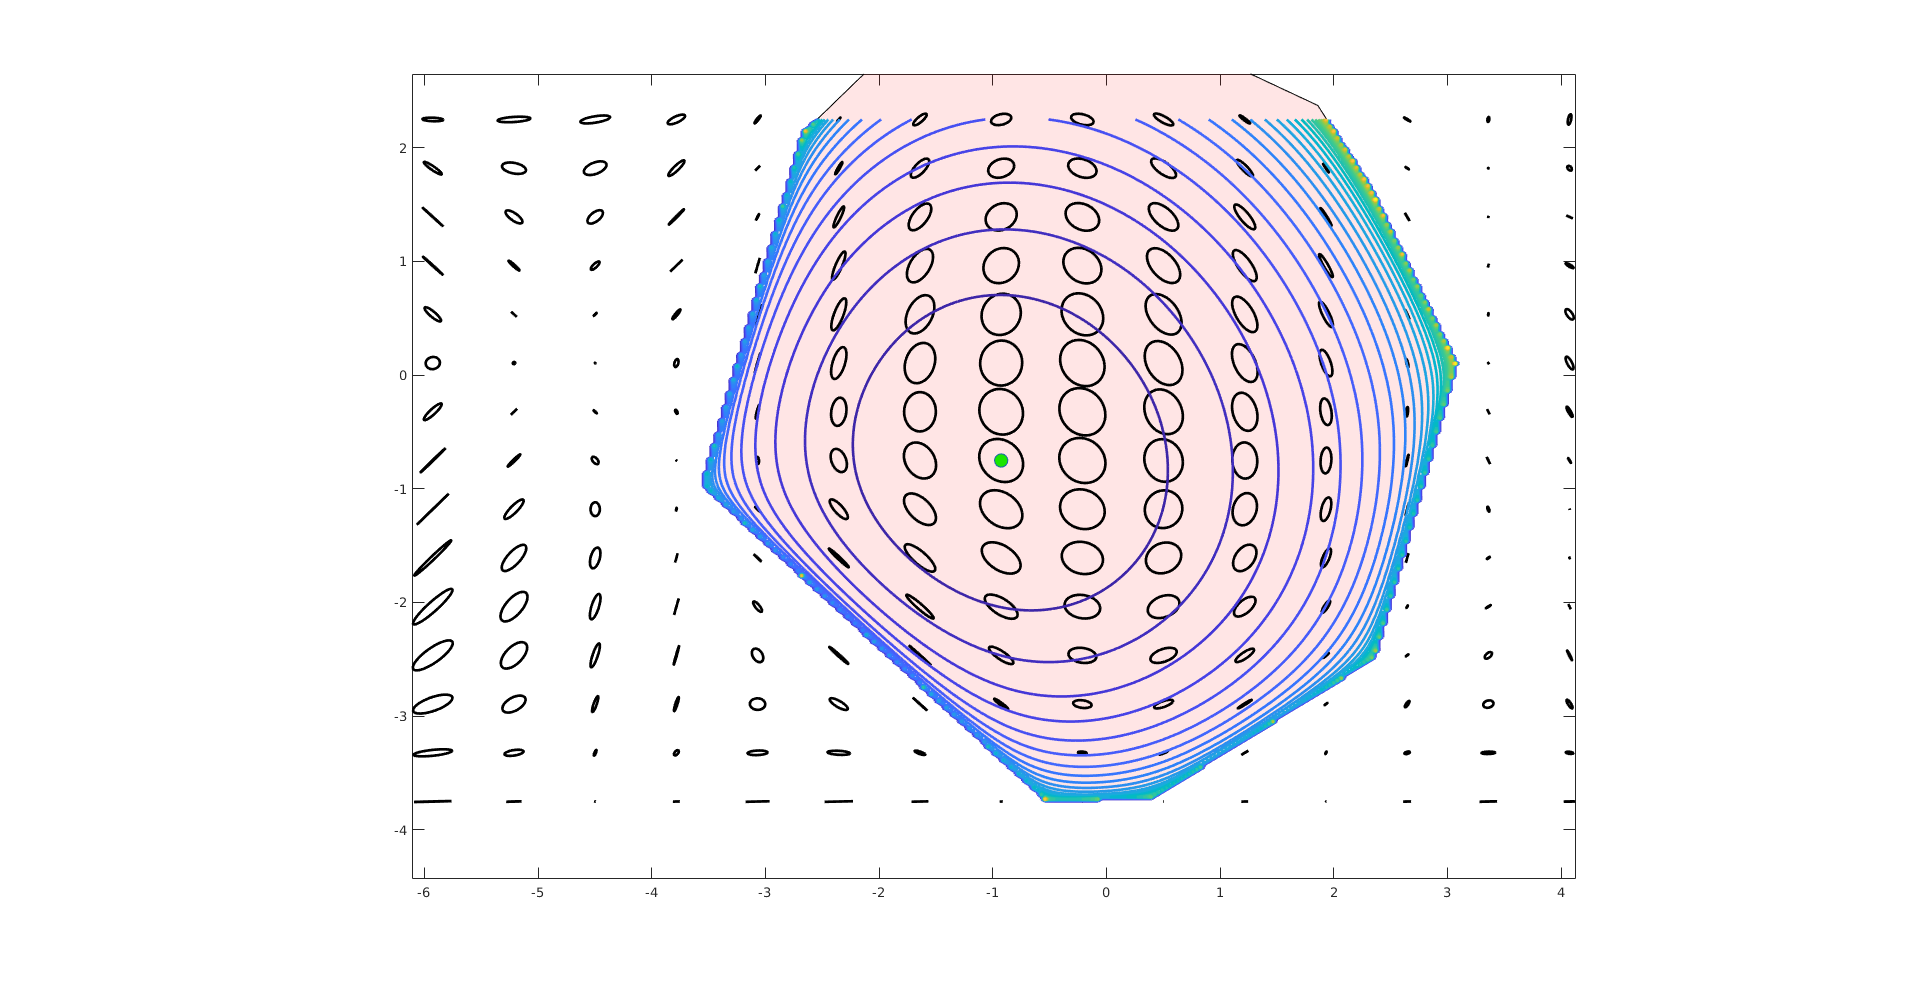
\includegraphics[width=\linewidth]{LogBarrier2.png}
    %\caption{Domain}
    \label{fig:BarrierFunctions}
\end{figure}

Pink is the domain. The ellipsoids represent the shape of the hessian $\frac{\partial^2 J}{\partial \bo{x}^2}$ at different points on the domain. Green dot is $\bo{x}_a$.

\end{flushleft}
\end{frame}










\myqrframe



\end{document}
